% alt + shift + 1
% make projname.pdf

\documentclass[12pt]{article}
%------------------------Dimensions----------------------------

\topmargin=0.0in
\oddsidemargin=0.0in           % 1in margins at left and right
\evensidemargin=0in
\textwidth=6.5in               % US paper is 8.5in wide
\marginparwidth=0.5in

\headheight=0pt                % 1in margins at top and bottom
\headsep=0pt
\topmargin=0in
\textheight=9.0in              % US paper is 11.0in high

%adjustments...
\addtolength{\topmargin}{-0.5in}
\addtolength{\textheight}{1.0in}
\addtolength{\textwidth}{0.5in}
\addtolength{\oddsidemargin}{-0.25in}
\addtolength{\evensidemargin}{-0.25in}
                       
\pagestyle{empty}

%------------------------Packages----------------------------
\usepackage{textcomp}
\usepackage{longtable}
\usepackage{setspace}
\usepackage{amsmath,amssymb,amsthm}
\usepackage{graphicx}
\usepackage{epsfig}
\usepackage{subfig}
\usepackage[paperwidth=8.5in,paperheight=11in,margin=0.98in]{geometry}
\usepackage{listings,float}
\usepackage{color}
\usepackage{array}
\usepackage{cancel}

%------------------------Commands----------------------------
\newcommand{\be}{\begin{enumerate}}
\newcommand{\ee}{\end{enumerate}}
\newcommand{\bi}{\begin{itemize}}
\newcommand{\ei}{\end{itemize}}
\newcommand{\bv} {{\bf v}}
\newcommand{\bD} {{\bf D}}

\newenvironment{definition}[1][Definition:]{\begin{trivlist}
\item[\hskip \labelsep {\bfseries #1}]}{\end{trivlist}}
\newenvironment{thm}[1][Theorem:]{\begin{trivlist}
\item[\hskip \labelsep {\bfseries #1}]}{\end{trivlist}}
\newenvironment{example}[1][Example]{\begin{trivlist}
\item[\hskip \labelsep {\bfseries #1}]}{\end{trivlist}}


\definecolor{listinggray}{gray}{0.9}
\definecolor{lbcolor}{rgb}{0.9,0.9,0.9}
\lstset{
	tabsize=4,
	rulecolor=,
	language=matlab,
	keywords={break,case,catch,continue,else,elseif,end,for,function,
      global,if,otherwise,persistent,return,switch,try,while},
        basicstyle=\footnotesize\ttfamily,
        upquote=true,
        aboveskip={1.5\baselineskip},
        columns=fixed,
        showstringspaces=false,
        extendedchars=true,
        breaklines=true,
        prebreak = \raisebox{0ex}[0ex][0ex]{\ensuremath{\hookleftarrow}},
        frame=single,
        showtabs=false,
        showspaces=false,
        showstringspaces=false,
        identifierstyle=\ttfamily,
        keywordstyle=\color[rgb]{0,0,1},
        commentstyle=\color[rgb]{0.133,0.545,0.133},
        stringstyle=\color[rgb]{0.627,0.126,0.941},
}

\captionsetup{width=.75\textwidth} 

\begin{document}
\pagestyle{plain} %pagenumbers
\title{CSCI 4/5576: Project Proposal \\ The Random Logistic Map}
\date{September 29, 2014}
\author{Amy Le (5576)\\Long Tat (4576)\\Emily Bertelson (4576)\\Kristina Entzel (4576)}
\maketitle

\section{Goal}
The purpose of this project is to characterize the Random Logistic
Map. In particular, we will be studying the stability of the map,
which includes locating fixed points and generating bifurcation
diagrams. As the map has an element of randomness to it, many
simulations (a large $N$) would be required for statistical analysis. This project is a subset of a larger work in progress. An
initial serial implementation has been developed and mildly tested in
MATLAB. The project would consist of converting the existing code to
C++ and implementing parallelization (OpenMP). Other possible improvements include
IO optimization and memory optimization.
\section{Background Information}
\subsection{Deterministic Logistic Map}
The Logistic map is a popularly studied topic in nonlinear
dynamics. The Logistic function is described as follows:
\begin{equation}\label{orig}
\hat{f}(x) = rx(1-x)
\end{equation}
where $r$ is a parameter that takes on values in [0,4]. To get the
Logistic Map, one simply discretizes the function by replacing
$\hat{f}(x)$ with $x_{n+1}$ and $x$ with $x_n$:
\begin{equation*}
x_{n+1}=rx_n(1-x_n)
\end{equation*}
\begin{figure}[H]
	\begin{center}
		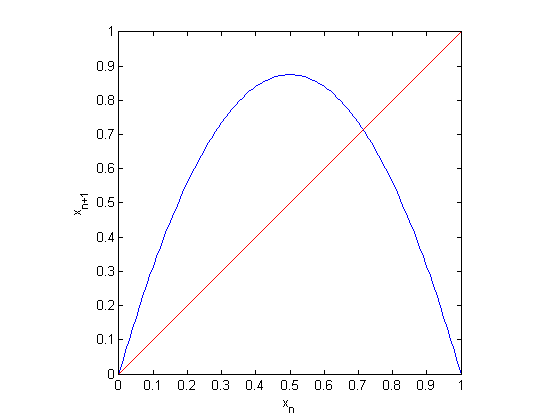
\includegraphics[scale=0.7]{deterministic}
	\end{center}
\end{figure}
Fixed points are located where the line $y=x$ intersects with the
Logistic Map. As the parameter $r$ is increased or decreased over the
interval [0,4], the map undergoes period doubling. Around $r=3.6$, the
map begins to display chaotic behavior.

\subsection{Random Logistic Map}
The Random Logistic function is a special case of the Logistic
function, which is not as popularly studied. In the random case, $r$ becomes a value dependent on $x$. Essentially, the Random Logistic
Map introduces the notion of spatial randomness to the deterministic
function (\ref{orig}). The Random Logistic function and map are as follows:
\begin{equation*}
f(x) = R(x)x(1-x)
\end{equation*}
\begin{equation}\label{randmap}
x_{n+1} = R(x_n)x_n(1-x_n)
\end{equation}
$R(x)$ consists of a Fourier series whose coefficients are independent
(but not identical) random variables drawn from a uniform
distribution. 
\begin{figure}[H]
	\begin{center}
		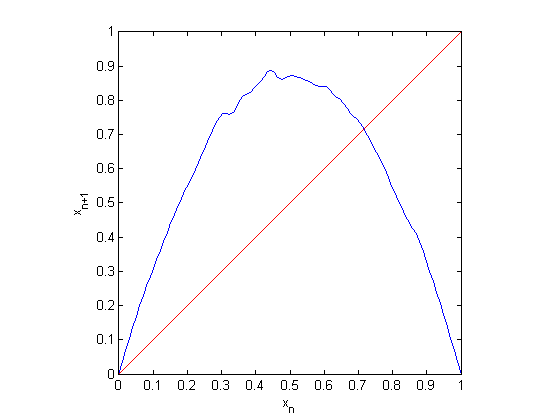
\includegraphics[scale=0.7]{random_cobweb}
	\end{center}
\end{figure}

\end{document}
